%%%
% Plantilla de Presentación
% Modificación de una plantilla de Latex de LaTeXTemplates para adaptarla 
% al castellano y a las necesidades de escribir informática y matemáticas.
%
% Editada por: Mario Román
%
% License:
% CC BY-NC-SA 3.0 (http://creativecommons.org/licenses/by-nc-sa/3.0/)
%%%

%%%%%%%%%%%%%%%%%%%%%%%%%%%%%%%%%%%%%%%%%
% Beamer Presentation
% LaTeX Template
% Version 1.0 (10/11/12)
%
% This template has been downloaded from:
% http://www.LaTeXTemplates.com
%
% License:
% CC BY-NC-SA 3.0 (http://creativecommons.org/licenses/by-nc-sa/3.0/)
%
%%%%%%%%%%%%%%%%%%%%%%%%%%%%%%%%%%%%%%%%%

%----------------------------------------------------------------------------------------
%   PAQUETES Y CONFIGURACIÓN DEL DOCUMENTO
%----------------------------------------------------------------------------------------

\documentclass{beamer}

%% Configuración de la presentación
\mode<presentation> {
  %%% Selección de estilo
  % The Beamer class comes with a number of default slide themes
  % which change the colors and layouts of slides. Below this is a list
  % of all the themes, uncomment each in turn to see what they look like.

  % \usetheme{default}
  % \usetheme{AnnArbor}
  % \usetheme{Antibes}
  % \usetheme{Bergen}
  % \usetheme{Berkeley} %% Esta plantilla mola un puñao
  % \usetheme{Berlin}
  % \usetheme{Boadilla}
  % \usetheme{CambridgeUS}
  % \usetheme{Copenhagen}
  % \usetheme{Darmstadt}
  \usetheme{Dresden}
  % \usetheme{Frankfurt}
  %\usetheme{Goettingen}
  %\usetheme{Hannover}
  %\usetheme{Ilmenau}
  %\usetheme{JuanLesPins}
  %\usetheme{Luebeck}
  % \usetheme{Madrid}
  % \usetheme{Malmoe}
  % \usetheme{Marburg}
  % \usetheme{Montpellier}
  %\usetheme{PaloAlto}
  %\usetheme{Pittsburgh}
  %\usetheme{Rochester}
  %\usetheme{Singapore}
  %\usetheme{Szeged}
  %\usetheme{Warsaw}

  %% Selección de color
  % As well as themes, the Beamer class has a number of color themes
  % for any slide theme. Uncomment each of these in turn to see how it
  % changes the colors of your current slide theme.

  % \usecolortheme{albatross}
  % \usecolortheme{beaver}
  %\usecolortheme{beetle}
  %\usecolortheme{crane}
  \usecolortheme{dolphin}
  %\usecolortheme{dove}
  %\usecolortheme{fly}
  %\usecolortheme{lily}
  %\usecolortheme{orchid}
  %\usecolortheme{rose}
  %\usecolortheme{seagull}
  %\usecolortheme{seahorse}
  %\usecolortheme{whale}
  %\usecolortheme{wolverine}

  %% Configuración del pie de línea
  %\setbeamertemplate{footline} % To remove the footer line in all slides uncomment this line
  %\setbeamertemplate{footline}[page number] % To replace the footer line in all slides with a simple slide count uncomment this line
  %\setbeamertemplate{navigation symbols}{} % To remove the navigation symbols from the bottom of all slides uncomment this line
}

%% Fuentes de tamaño arbitrario
\usepackage{lmodern}

%% Gráficos
\usepackage{graphicx} % Allows including images
\usepackage{booktabs} % Allows the use of \toprule, \midrule and \bottomrule in tables

%% Colors
\usepackage{color}

%%% Castellano.
% noquoting: Permite uso de comillas no españolas.
% lcroman: Permite la enumeración con numerales romanos en minúscula.
% fontenc: Usa la fuente completa para que pueda copiarse correctamente del pdf.
% \usepackage[spanish,es-noquoting,es-lcroman]{babel}
\usepackage[utf8]{inputenc}
\usepackage[T1]{fontenc}
% \selectlanguage{spanish}

%----------------------------------------------------------------------------------------
%   TÍTULO
%----------------------------------------------------------------------------------------

\title[Telegram, secure messaging]{Telegram, secure messaging} % The short title appears at the bottom of every slide, the full title is only on the title page
\subtitle{
\includegraphics[scale=0.15]{images/t_logo}}
\author{Francisco Luque Sánchez - María de Mar Ruiz Martín} % Your name
\institute[UGR] % Your institution as it will appear on the bottom of every slide, may be shorthand to save space
{
  Universidad de Granada \\ % Your institution for the title page
  \medskip
  \textit{fluque1995@correo.ugr.es - mariadel52@correo.ugr.es}\\ % Your email address
}
\date{\today} % Date, can be changed to a custom date



\begin{document}

%% Diapositiva de título.
\begin{frame}
\titlepage % Print the title page as the first slide
\end{frame}

%% Diapositiva de contenidos.
% Throughout your presentation, if you choose to use \section{} and \subsection{} commands, 
% these will automatically be printed on this slide as an overview of your presentation
\begin{frame}
  \frametitle{Presentation index} % Table of contents slide, comment this block out to remove it
  \tableofcontents
\end{frame}



%----------------------------------------------------------------------------------------
%   PRESENTACIÓN
%----------------------------------------------------------------------------------------

%------------------------------------------------
\section{Introduction} % Sections can be created in order to organize your presentation into discrete blocks, all sections and subsections are automatically printed in the table of contents as an overview of the talk
%------------------------------------------------

\begin{frame}
\frametitle{Introduction}
Telegram is a safe instant messaging application. Features:
\begin{itemize}
\item Secure
\item Encrypted
\item Own transport protocol (MTProto)
\item Multiplatform
\item Cloud-based
\item Open source
\item Powerful APIs (provided by Telegram team)
\item Free "forever"
\end{itemize}
\end{frame}

%------------------------------------------------
\section{Telegram security}
%------------------------------------------------

\begin{frame}
\frametitle{Telegram security}
Telegram uses different features for secure messaging and message encryption
\begin{itemize}
\item MTProto message encryption
\item Private chatting
\begin{itemize}
\item End-to-end encrypted messages
\item Self-destruction for messages
\end{itemize}
\end{itemize}
\end{frame}

%------------------------------------------------
\subsection{MTProto}
%------------------------------------------------

\begin{frame}
\frametitle{MTProto protocol}
Transport and encryption protocol created by Telegram team (invented by Nikolai Durov, PhD Saint Pertersbourg Univ.).
Based on:
\begin{itemize}
\item 256-bits symmetric AES encryption
\item RSA 2048 encryption
\item Diffie-Hellman key exchange
\end{itemize}
It allows multi-platform usage and file sending in every format
\href{https://core.telegram.org/mtproto/description}{\color{blue}MTProto detailed description} \\
Telegram haking contest: They will pay 300000 \$ to the Telegram Encryption cracker
\end{frame}

\subsubsection{Protocol Schema}

\begin{frame}
\frametitle{MTProto encryption schema}
\begin{center}
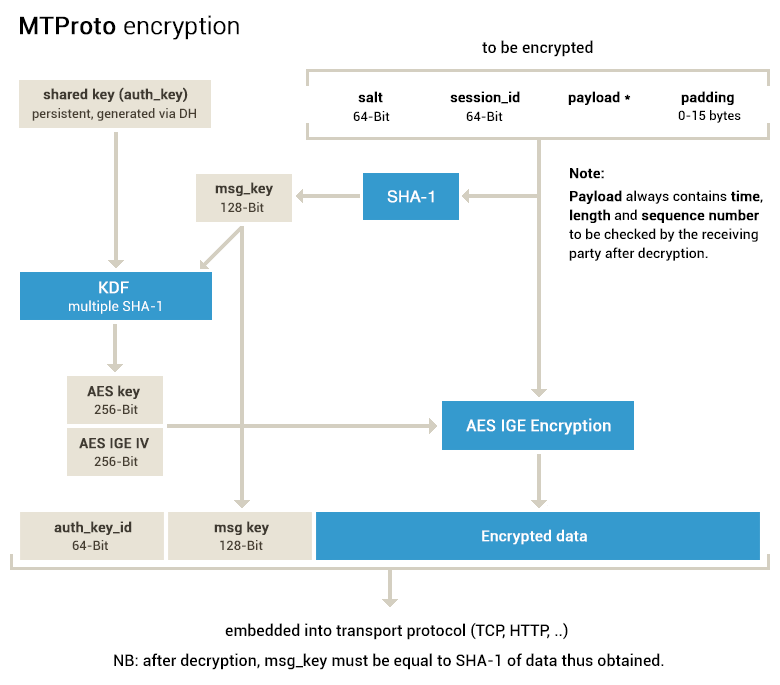
\includegraphics[scale=0.25]{images/mtproto_schema}
\end{center}
\end{frame}
%------------------------------------------------
\begin{frame}
\frametitle{End-to-end encrypted messages - secret chats}
Completely secure chats \\~\\
Messages encrypted end-to-end (Encrypted by sender and decrypted by receiver) \\~\\
No one is allowed to see the content of those messages, including Telegram team \\~\\
They are not stored in Telegram cloud (you will only have access from the device
of origin or destiny) \\~\\
News: \href{http://abcnews.go.com/Technology/wireStory/telegram-ceo-app-blocked-iran-surveillance-request-34644937}{\color{blue}Iran blocked Telegram App after spy request}
\end{frame}

\begin{frame}
\frametitle{Self destruction for messages}
Secret chat feature\\~\\
Messages and files are deleted after a period of time\\~\\
They are deleted from sender and receiver\\~\\
Not stored on their servers\\~\\
\begin{center}
Everything you delete is deleted forever. Except for cats.\\
We never delete your funny cat pictures, we love them too much.\\~\\
Telegram developer team
\end{center}
\end{frame}

%------------------------------------------------
\section{Open Source and APIs}
%------------------------------------------------

\begin{frame}
\frametitle{Open Source and APIs}
Almost the whole code is open source, except for some code from the server (Keep calm! They promise they will release it soon)\\~\\
APIs for applications and Bots\\~\\
\end{frame}

%------------------------------------------------

\begin{frame}
\frametitle{Application API}
Wonderful client application API\\~\\
They give us everything we need to create our own Telegram client\\~\\
\href{https://core.telegram.org/\#telegram-api}{\color{blue}Telegram API documentation}\\~\\
Code of official Apps is released on github\\~\\
\href{https://github.com/DrKLO/Telegram}{\color{blue}Android App code}\\~\\
\end{frame}

%------------------------------------------------

\begin{frame}
\frametitle{Bots API}
\begin{columns}
\column{.75\textwidth}
Community started creating bots not supported by Telegram\\~\\
Due to fast success of some of them, they decided to create an official Bots API\\~\\
Now, Bots are really powerful tools \\~\\
\href{https://github.com/acasadoquijada/ETSIIT_BOT}{\color{blue}ETSIIT Bot source code}\\~\\
Q: What can I do with bots?\\~\\
Telegram: Do virtually anything. Except for dishes — bots are terrible at doing the dishes.
\column{.25\textwidth}

\includegraphics[scale=0.5]{images/botfather}
\end{columns}
\end{frame}

%------------------------------------------------

\begin{frame}
\Huge{\centerline{The End.}}
\large{\centerline{github repository: \href{https://github.com/pacron/telegram_beamer}{\color{blue}https://github.com/pacron/telegram\_beamer}}}
\end{frame}

%----------------------------------------------------------------------------------------

\end{document} 